\documentclass{article}

\usepackage{siunitx} % Provides the \SI{}{} and \si{} command for typesetting SI units
\usepackage{graphicx} % Required for the inclusion of images
\usepackage{amsmath} % Required for some math elements 
\usepackage[export]{adjustbox} % loads also graphicx
\usepackage{listings}
\usepackage{matlab-prettifier}
\usepackage{float}
\usepackage[most]{tcolorbox}
\usepackage{amsfonts}
\usepackage{color}
\usepackage{titlesec}
\usepackage{caption}
\usepackage{subcaption}
\usepackage{placeins}

\newcommand{\R}{\mathbb{R}}

\usepackage{xcolor}

\DeclareCaptionFont{white}{\color{white}}
\DeclareCaptionFormat{listing}{%
  \parbox{\textwidth}{\colorbox{gray}{\parbox{\textwidth}{#1#2#3}}\vskip-4pt}}
\captionsetup[lstlisting]{format=listing,labelfont=white,textfont=white}
\lstset{frame=lrb,xleftmargin=\fboxsep,xrightmargin=-\fboxsep}
\titleformat{\section}[runin]
  {\normalfont\Large\bfseries}{\thesection}{1em}{}
\titleformat{\subsection}[runin]
  {\normalfont\large\bfseries}{\thesubsection}{1em}{}


\setlength\parindent{0pt} % Removes all indentation from paragraphs

\renewcommand{\labelenumi}{\alph{enumi}.} % Make numbering in the enumerate environment by letter rather than number (e.g. section 6)

%\usepackage{times} % Uncomment to use the Times New Roman font

%----------------------------------------------------------------------------------------
%	DOCUMENT INFORMATION
%----------------------------------------------------------------------------------------

\title{AMATH 353: Homework 14 \\Due May, 30 2018 \\ ID: 1064712} % Title

\author{Trent \textsc{Yarosevich}} % Author name

\date{\today} % Date for the report

\begin{document}
\maketitle % Insert the title, author and date
\setlength\parindent{1cm}

\begin{center}
\begin{tabular}{l r}
%Date Performed: December 1, 2017 \\ % Date the experiment was performed
Instructor: Jeremy Upsal % Instructor/supervisor
\end{tabular}
\end{center}

% If you wish to include an abstract, uncomment the lines below
% \begin{abstract}
% Abstract text
% \end{abstract}

%----------------------------------------------------------------------------------------
%	SECTION 1
%----------------------------------------------------------------------------------------
\section*{Part 1}
\subsection*{(a)}
Given the following initial condition, we get:
\begin{equation}
u(x,0)= 
  \begin{cases}
			\frac{\pi}{2}, \; \; \; x < 1 \\
			\frac{\pi}{4}, \; \; \; x \geq 1 \\
            \end{cases}
\
\end{equation}
\begin{equation}
\begin{aligned}
\frac{du}{dt} = 0\\
u(x(t), t) = A\\
A = u_0(x_0) = u(x, 0)\\
\end{aligned}
\end{equation}
We can then make use of $x(t) = x_0 + c(u_0(x_0)t$: and determine the equations for the characteristics:
\begin{equation}
\begin{aligned}
c(u(x(t), t)) = \sin(u)\\
c(u_0(x_0) = \sin(u_0(x_0))\\
\end{aligned}
\end{equation}
\begin{equation}
c(u_0(x_0) 
  \begin{cases}
			1, \; \; \; x_0 < 1 \\
			\frac{\sqrt{2}}{2}, \; \; \; x_0 \geq 1 \\
            \end{cases}
\
\end{equation}
This in turn gives the following characteristics curves:
\begin{equation}
x(t) = 
  \begin{cases}
			x_0 + t, \; \; \; x_0 < 1 \\
			x_0 + \frac{\sqrt{2}}{2}t, \; \; \; x_0 \geq 1 \\
            \end{cases}
\
\end{equation}
\begin{equation}
t = 
  \begin{cases}
			x - x_0, \; \; \; x_0 < 1 \\
			\sqrt{2}(x - x_0) \; \; \; x_0 \geq 1 \\
            \end{cases}
\
\end{equation}
Additionally, here are the functions of $x_0$ in terms of $x$ and $t$, which will be useful later:
\begin{equation}
x_0 =
  \begin{cases}
			x - t, \; \; \; x_0 < 1 \\
			x - \frac{\sqrt{2}}{2}t \; \; \; x_0 \geq 1 \\
            \end{cases}
\
\end{equation}
\subsection*{(b)}
Because $u(x(t), t) = u_0(x_0)$ we can find the breaking time by finding where its derivative goes to $\infty$. 
\begin{equation}
u_x = u_0'(x_0)\frac{dx_0}{dx}\\
\end{equation}
It is clear from the initial condition given above that we cannot take the derivative $u_0'(x_0)$ because $u_0(x_0)$ has a discontinuity when $x_0 = 1$. Plugging this into equation (7) above at $t=0$ we see that this occurs at $x = 1$.
\subsection*{(c)}
Since $\phi(x,t) = \sin(u)u_x$ we can integrate to get the following (note that I am ignoring the constant of integration, since it drops out in the Rankine-Hugoniot relation anyway):
\begin{equation}
\phi(x, t) = -\cos(u)
\end{equation}
We know from equation (2) above that $u^- = \frac{\pi}{2}$ and $u^+ = \frac{\pi}{4}$ giving:
\begin{equation}
\begin{aligned}
\frac{dx_s}{dt} = \frac{[\phi]}{[u]}\\
\frac{[\phi]}{[u]} = \frac{-\cos(u^+) + \cos(u^-)}{u^+ - u^-}\\
\frac{dx_s}{dt} = \frac{-\frac{\sqrt{2}}{2}}{-\frac{\pi}{4}}
\end{aligned}
\end{equation}
Which simplifies to:
\begin{equation}
\frac{dx_s}{dt} = \frac{2\sqrt{2}}{\pi}
\end{equation}
We then integrate and apply the initial condition found in (b):
\begin{tcolorbox}[minipage,colback=white,arc=0pt,outer arc=0pt]
\begin{equation}
\begin{aligned}
x_s(t) = \frac{2\sqrt{2}}{\pi}t + C\\
x_s(0) = 1 = C\\
x_s(t) = \frac{2\sqrt{2}}{\pi}t + 1
\end{aligned}
\end{equation}
\end{tcolorbox}
\begin{figure}[!htbp]
  \centering
    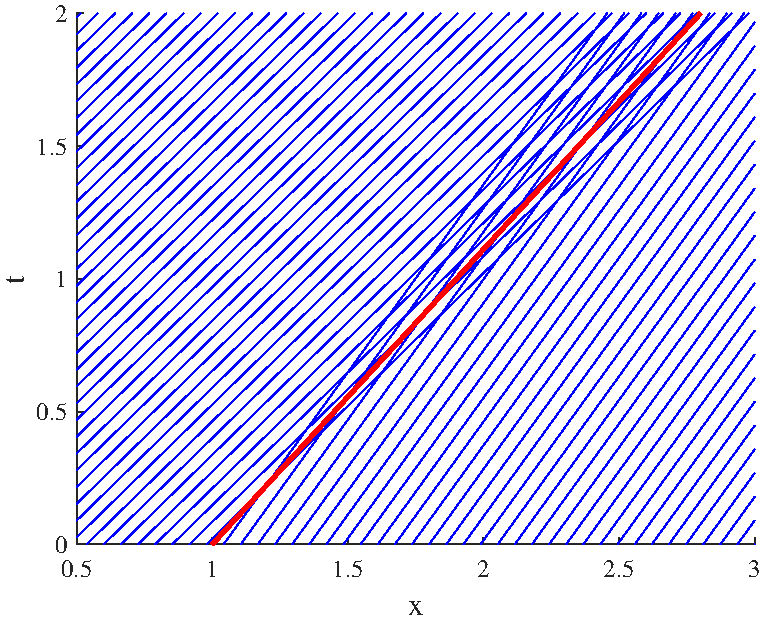
\includegraphics[width=\textwidth]{hw_14_plot1.pdf}
    \caption{Characteristics and $x_s$}
\end{figure}
\FloatBarrier
\subsection*{(d)}
The solution to the left of the shockline is a line at $u = \frac{\pi}{2}$, and to the right, a line at $u = \frac{\pi}{4}$. This is defined as: 
\begin{tcolorbox}[minipage,colback=white,arc=0pt,outer arc=0pt]
\begin{equation}
u(x,t) =
  \begin{cases}
			\frac{\pi}{2}, \; \; \; x < x_s \\
			\frac{\pi}{4} \; \; \; x \geq x_s \\
            \end{cases}
\
\end{equation}
\end{tcolorbox}
\subsection*{(e)}
If we change the characteristics in this way,the density increases at the discontinuity, so the speed for $u^+$ is actually greater than $u^-$. As a result, the space between the solutions for $u$ actually increases in time, giving a growing region in which $u$ is not defined.
\begin{figure}[!htbp]
  \centering
    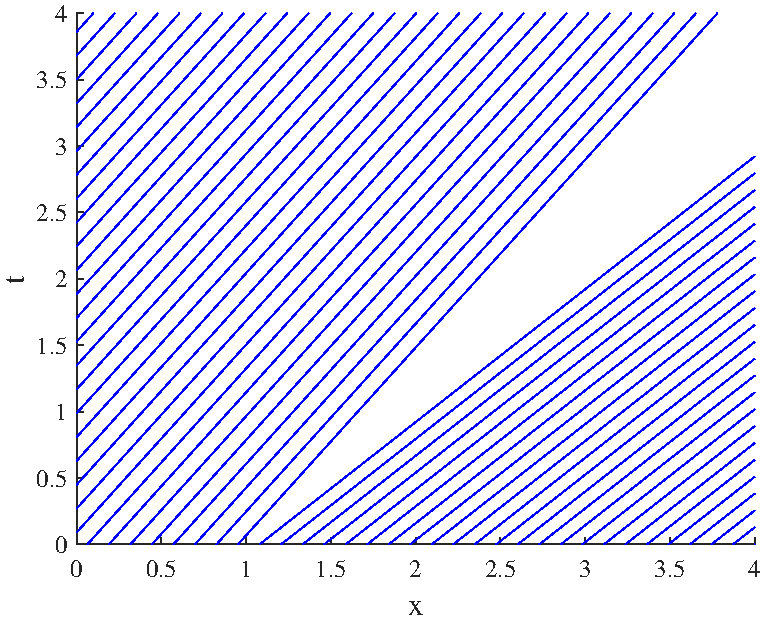
\includegraphics[width=\textwidth]{hw_14_plot2.pdf}
    \caption{$u^-=\frac{\pi}{4}$ and $u^+=\frac{\pi}{2}$}
\end{figure}
\FloatBarrier
\section*{Part 2}
\subsection*{(a)}
\begin{figure}[!htbp]
  \centering
    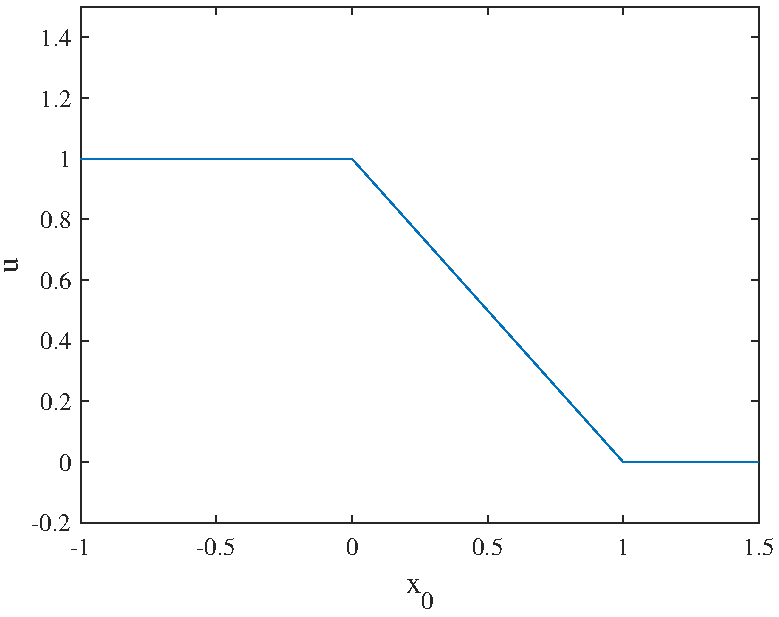
\includegraphics[width=\textwidth]{hw_14_plot3.pdf}
    \caption{$u(x, 0)$}
\end{figure}
\FloatBarrier
\subsection*{(b)}
First, we obtain the solution to $u$ along the characteristics:
\begin{equation}
\begin{aligned}
\frac{du}{dt} = 0\\
u(x(t), t) = A\\
A = u(x,0) = u_0(x_0)\\
\end{aligned}
\end{equation}
\begin{equation}
u(x(t),t) =
  \begin{cases}
			1, \; \; \; x_0 \leq 0 \\
			1-x_0, \; \; \; 0 < x_0 < 1\\
			0, \; \; \; x_0 \geq 1\\
            \end{cases}
\
\end{equation}
Using the values for $u_0(x_0)$ and $x(t) = x_0 + c(u_0(x_0))t$, we then obtain the characteristic curves:
\begin{tcolorbox}[minipage,colback=white,arc=0pt,outer arc=0pt]
\begin{equation}
x(t) =
  \begin{cases}
			x_0 + t, \; \; \; x_0 \leq 0 \\
			x_0 + t(1-x_0), \; \; \; 0 < x_0 < 1\\
			x_0, \; \; \; x_0 \geq 1\\
            \end{cases}
\
\end{equation}
\end{tcolorbox}
d
\end{document}